\documentclass{scrartcl}
\usepackage[utf8]{inputenc}
\usepackage{hyperref}
\usepackage{url}
\usepackage{natbib}
\usepackage{graphicx}
\usepackage{listings}
\usepackage{xcolor}
\usepackage{paralist}
\usepackage{enumitem}

\definecolor{dkgreen}{rgb}{0,0.6,0}
\definecolor{gray}{rgb}{0.5,0.5,0.5}
\definecolor{mauve}{rgb}{0.58,0,0.82}

\lstdefinestyle{scalaStyle}{
  frame=tb,
  language=scala,
  aboveskip=3mm,
  belowskip=3mm,
  showstringspaces=false,
  basicstyle=\ttfamily\footnotesize,
  numbers=left,
  numberstyle=\tiny\color{gray},
  keywordstyle=\color{blue},
  commentstyle=\color{dkgreen},
  stringstyle=\color{mauve},
  frame=single,
  breaklines=true,
  breakatwhitespace=true
}

\lstset{style=scalaStyle}

\newcommand{\emailaddr}[1]{\href{mailto:#1}{\texttt{#1}}}

\title{\LARGE
    PPS Final Report
}

\author{
    Davide Evangelisti \\ \emailaddr{davide.evangelisti2@studio.unibo.it}
    \and 
    Francesco Dente \\ \emailaddr{francesco.dente@studio.unibo.it} 
    \and 
    Shapour Nemati \\ \emailaddr{shapour.nemati@studio.unibo.it}
    \and 
    Simone Magnani \\ \emailaddr{simone.magnani4@studio.unibo.it} 
    
}

\date{\today}

\begin{document}

\maketitle

\tableofcontents

\newpage

\section*{Introduzione}
Questo report è relativo allo sviluppo della libreria SBAGS e dei seguenti giochi: TicTacToe, Connect Four ed Othello.
%
La libreria permette di realizzare giochi di strategia astratti basati su scacchiera, descrivendo alcuni aspetti statici e strutturali tramite i costrutti propri del linguaggio scala, e gli aspetti più dinamici tramite un DSL in un linguaggio simil-naturale.
%
SBAGS ha come target principale giochi in cui due o più giocatori interagiscono a turni alterni, spostando pedine sulle tessere di una scacchiera e seguendo un insieme di regole ben definite fino a quando non viene raggiunto uno stato terminale.
%
Alcuni esempi di questi giochi sono Scacchi, Dama, TicTacToe, Connect Four ed Othello.

Se un utente desidera realizzare un gioco con caratteristiche convenzionali dovrà svolgere uno sforzo minimo, infatti per il caso di board rettanglare viene generata automaticamente dalla libreria un'interfaccia grafica testuale.
%
Qualora il gioco da realizzare risulti necessitare feature non presenti nella libreria questa sarà comunque espandibile direttamente dall'utente, che potrà integrare le nuove funzionalità a quelle già presenti seguendo una struttura già definita, ottenendo così la possibilità di godere di tutte le caratteristiche di entrambi.

\addcontentsline{toc}{section}{Introduzione}

\newpage

\section{Processo di sviluppo}

% (modalità di divisione in itinere dei task, meeting/interazioni pianificate, modalità di revisione in itinere dei task, scelta degli strumenti di test/build/continuous integration)


\newpage

\section{Requisiti}

Questa sezione è redatta considerando come utenti i programmatori che utilizzeranno la libreria per sviluppare i giochi, mentre i requisiti dei giocatori che utilizzeranno il software costruito adoperando questa libreria non sono considerati rilevanti.

\subsection{Business}

La libreria consentirà di realizzare giochi da tavolo con le seguenti caratteristiche:
%
\begin{enumerate}
    \item Requisiti di business.
    \begin{enumerate}[label*=\arabic*.]
        \item Giochi basati sul movimento di pedine all'interno di un tabellone;
        \item Giochi a informazione perfetta\footnote{\url{https://it.wikipedia.org/wiki/Gioco_a_informazione_completa}};
        \item Giochi in cui è necessario gestire lo sviluppo della partita (turni, condizioni di vittoria, vincitore della partita, \dots).
    \end{enumerate}
\end{enumerate}

In paricolare deve essere possibile realizzare i seguenti giochi:
%
\begin{enumerate}[resume]
    \item Giochi sviluppati.
    \begin{enumerate}[label*=\arabic*.]
        \item ``\textbf{Put-In-Put-Out}'': un gioco dove l'utente può piazzare e rimuovere una pedina sull'unica casella del tabellone, senza ulteriori funzionalità;
        %
        \item ``\textbf{TicTacToe}'': il gioco del tris, in cui a turno due giocatori piazzano in una casella di una matrice 3x3 il proprio simbolo (solitamente una X e una O).
        %
        Vince il giocatore che riesce a disporre tre delle proprie pedine in linea retta orizzontale, verticale o diagonale.
        %
        Se la matrice viene riempita senza che nessun sia riuscito a creare un tris, il gioco finisce in parità;
        %
        \item ``\textbf{Connect Four}'': Forza4 è un gioco basato su tabellone, in particolare una matrice 6x7, all'interno del quale si possono posizionare delle pedine solo nella prima casella libera di ogni colonna.
        %
        In particolare due giocatori, in modo alternato, inseriscono uno delle proprie pedine all'interno di una colonna.
        %
        Il vincitore è colui che riesce a disporre quattro delle proprie pedine adiacenti in linea retta orizzontale, verticale o diagonale.
        %
        Nel caso di riempimento del tabellone senza che nessun giocatore sia riuscito a vincere, il gioco finisce in parità;
        %
        \item ``\textbf{Othello}'': un gioco basato su una scacchiera 8x8 chiamata othelliera.
        %
        Il gioco prevede la presenza di due giocatori ai quali è assegnato un colore (solitamente bianco e nero). 
        %
        Il gioco inizia con due pedine per giocatore poste nelle caselle centrali a formare una 'X'.
        %
        I turni dei giocatori sono alternati; in ogni turno un giocatore può posizionare una sua pedina in modo da imprigionare una o più pedine dell'avversario tra quella posizionata ed altre sue pedine.
        %
        Ogni pedina imprigionata diventa del giocatore di turno. 
        %
        In mancanza di mosse disponibili il giocatore deve passare il turno.
        %
        L'obiettivo del gioco è di avere più pedine dell'avversario sull'othelliera quando non ci sono più mosse disponibili o quando l'othelliera è piena.
    \end{enumerate}
\end{enumerate}

%------------------------------------------------------------------------------------
\subsection{Utente}

Uno sviluppatore che utilizzerà la libreria dovrà fornire una specifica del gioco utilizzando i costrutti messi a disposizione dalla stessa, e successivamente potrà usufruire del gioco generato da tali specifiche tramite degli appositi comandi.
%
In particolare l'utente può definire i seguenti aspetti:
%
\begin{enumerate}[resume]
    \item Requisiti utente.
    \begin{enumerate}[label*=\arabic*.]
        \item rappresentazione delle pedine all'interno del gioco;
        \item rappresentazione delle celle e del modo in cui compongono il tabellone;
        \item rappresentazione delle mosse;
        \item rappresentazione dello stato del gioco;
        \item regole del gioco:
        \begin{enumerate}[label*=\arabic*.]
            \item con API classica o tramite DSL interno;
            \item generazione delle mosse disponibili a partire da un dato stato di gioco;
            \item definizione delle azioni che vengono eseguite sullo stato del gioco a fronte dell'esecuzione di una mossa;
        \end{enumerate}
        \item descrizione del gioco, che prevede:
        \begin{enumerate}[label*=\arabic*.]
            \item definizione dello stato del gioco iniziale;
            \item definizione di eventuali estensioni del gioco:
            \begin{enumerate}[label*=\arabic*.]
                \item giocatori che partecipano a una partita;
                \item flusso dei turni;
                \item condizioni di terminazione;
            \end{enumerate}
        \end{enumerate}
        \item interazione tramite UI, definendo:
        \begin{enumerate}[label*=\arabic*.]
            \item il tipo di UI utilizzata tra le seguenti:
            \begin{enumerate}[label*=\arabic*.]
                \item \label{req:cli} interfaccia testuale (CLI), fornita dalla libreria;
                \item \label{req:custom_view} interfaccia personalizzata, definita dall'utente;
            \end{enumerate}
            \item \label{req:renderers_parameters} i parametri necessari alla UI per effettuare il display dello stato del gioco;
            \item \label{req:events} i parametri per la conversione degli eventi generati dalla UI in mosse da eseguire sul gioco;
        \end{enumerate}
    \end{enumerate}
\end{enumerate}

\subsection{Funzionali}

La libreria implementerà le funzionalità base che, opportunamente composte, costituiranno un gioco con un determinato insieme di regole.

La libreria dovrà:
%
\begin{enumerate}[resume]
    \item Requisiti funzionali.
    \begin{enumerate}[label*=\arabic*.]
        \item supportare diversi tipi di pedine, a patto che abbiamo uno specifico sopratipo comune;
        \item supportare diversi tipi di caselle, a patto che abbiamo uno specifico sopratipo comune;
        \item \label{req:board_state} supportare diversi tipi di tabelloni:
        \begin{enumerate}[label*=\arabic*.]
            \item fornendo astrazioni di base per i tabelloni comuni (e.g. rettangolari, quadrati, \dots);
            \item lasciando la possibilità allo sviluppatore di rappresentare strutture personalizzate;
        \end{enumerate}
        \item fornire le seguenti azioni sul tabellone:
        \begin{enumerate}[label*=\arabic*.]
            \item inserimento di una pedina su una casella;
            \item rimozione di una pedina da una casella;
            \item lettura dello stato di una casella, ovvero quale eventuale pedina vi è posizionata sopra;
            \item azioni composite, derivate da una sequenza arbitraria delle precedenti;
        \end{enumerate}
        \item gestire lo svolgersi di una partita:
        \begin{enumerate}[label*=\arabic*.]
            \item permettendo di verificare in ogni momento se una mossa è valida;
            \item permettendo di ottenere l'insieme di tutte le mosse valide in un dato istante; 
            \item impedendo l'esecuzione di mosse illegali;
            \item aggiornando lo stato corrente all'esecuzione di una mossa valida, seguendo quanto indicato dalle regole;
            \item \label{req:end_game_cond} rilevando la terminazione della partita;
            \item \label{req:undo} permettendo di annullare una mossa eseguita, mantenendo una cronologia della partita;
        \end{enumerate}
        \item \label{req:dsl} fornire un DSL per la scrittura delle regole, che offre una sintassi semplificata e in linguaggio simil-naturale per:
        \begin{enumerate}[label*=\arabic*.]
            \item \label{req:action} eseguire azioni che modificano lo stato del gioco:
            \begin{enumerate}[label*=\arabic*.]
                \item inserimento di pedine;
                \item rimozione di pedine;
                \item spostamento di pedine;
                \item rimpiazzo di pedine;
                \item avanzamento del turno;
                \item altre azioni personalizzate;
            \end{enumerate}
            \item \label{req:generator} definire le regole per generare le mosse disponibili in un dato momento;
            \item concatenare le istruzioni di base, per creare azioni composite o sequenze di generatori;
            \item iterare sulle proprietà dello stato del gioco;
            \item verificare condizioni sullo stato del gioco;
            \item \label{req:iterating} innestare i costrutti iterativi e condizionali.
        \end{enumerate}
    \end{enumerate}
\end{enumerate}

\subsection{Non funzionali}

Data la natura del software prodotto, la sua dipendenza dal codice degli utenti che ne faranno utilizzo, e la mancanza di elementi distribuiti, non sono individuati requisiti non funzionali.
%
Questi sono lasciati agli utilizzatori della libreria che dovranno calibrarli in base al tipo di applicazione e di utente.

\subsection{Di implementazione}

La libreria dovrà essere sviluppata in Scala, e verranno svolti dei test con \textbf{Scalatest} per minimizzare la presenza di errori e facilitare l'aggiornamento di eventuali funzionalità.

\newpage

\section{Analisi del dominio}

Il risultato dell'analisi del dominio dei giochi da tavolo è rappresentato in Figura \ref{fig:domain_analysis}.
%
L'analisi ha evidenziato la presenza costante di una divisione in \textbf{aspetti intensionali}, ovvero fissati indipendentemente da una specifica partita, ed \textbf{aspetti estensionali}, che catturano dettagli legati al gioco durante il suo svolgimento.

\begin{figure}
  \centering
  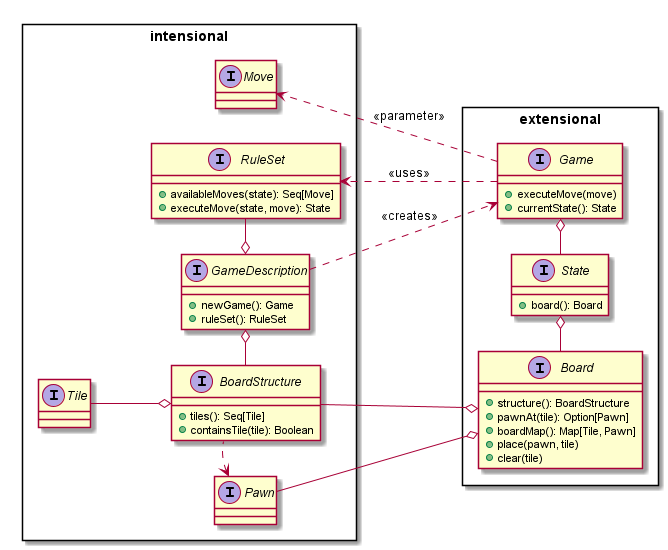
\includegraphics[width=\linewidth]{images/uml/domain_analysis.png}
  \caption{Diagramma delle classi rappresentante il risultato dell'analisi del modello del dominio}
  \label{fig:domain_analysis}
\end{figure}

\subsection{Aspetti intensionali}
I concetti intensionali sono visibili nella porzione di sinistra del diagramma in Figura \ref{fig:domain_analysis}.

Il nucleo di questo insieme di entità è costituito dalla \texttt{GameDescription}, che rappresenta la definizione principale di un gioco e viene utilizzata per crearne nuove istanze.
%
Ad ogni \texttt{GameDescription} è associato un \texttt{RuleSet}, che contiene la logica per la generazione e l'esecuzione delle mosse disponibili per un dato stato della partita, e una \texttt{BoardStructure} contenente la disposizione dei \texttt{Tile} che costituiscono il tabellone di gioco e il tipo di \texttt{Pawn} che possono ospitare.

Infine, fanno parte degli aspetti intensionali anche le \texttt{Move}, che racchiudono tutte le informazioni necessarie al \texttt{RuleSet} per l'esecuzione della mossa stessa.

\subsection{Aspetti estensionali}
A livello estensionale, le entità individuate sono collocate nella metà di destra del diagramma in Figura \ref{fig:domain_analysis}.

La radice di questo gruppo di entità è il \texttt{Game}, ovvero la rappresentazione di una istanza attiva di partita.
%
Ad esso è affidato il compito di mantenere consistente lo \texttt{State} della partita a fronte dell'esecuzione delle \texttt{Move} e utilizza quindi il \texttt{RuleSet} per garantire questa proprietà.

Uno \texttt{State} contiene tutte le informazioni necessarie a definire un istante legale del proseguimento della partita, comprendente di stato della \texttt{Board}, giocatori attivi, turno corrente, ecc.
%
Non tutti questi aspetti sono condivisi da tutti i giochi da tavolo, e sono perciò omessi nel diagramma ad eccezione della \texttt{Board}, che è sempre presente.

Infine, la \texttt{Board} è l'entità che definisce e manovra la disposizione dei \texttt{Pawn} sui \texttt{Tile} definiti dalla sua \texttt{BoardStructure}.
%
La \texttt{Board} deve anche imporre il vincolo di avere al più un \texttt{Pawn} su ogni \texttt{Tile}.

\subsection{Aspetti comuni dei giochi da tavolo}
%
Si analizzano ora gli aspetti trasversali a tutti i giochi da tavolo.
%
\paragraph{Turni e Giocatori}
%
I giochi da tavolo sono quasi sempre suddivisi in turni che scandiscono il flusso di una partita; un turno solitamente identifica una serie di azioni le quali possono essere svolte prima della sua terminazione.
%
Ogni gioco, inoltre, ha un numero fissato di giocatori che prendono parte ad una partita (un gioco con zero giocatori è da intendersi come un simulatore e non più un gioco).
%
Il sistema dei turni e quello dei giocatori sono quasi sempre fortemente legati tra loro e in molti casi i concetti di turno e di giocatore sono sovrapposti e interscambiabili.
%
\paragraph{Condizioni di terminazione}
%
Queste identificano l'insieme di condizioni necessarie e sufficienti affinchè una partita termini.
%
Le partite possono terminare solitamente in due modi:
\begin{itemize}
  \item vittoria di un giocatore: caso in cui un giocatore ha raggiunto i requisisti per essere dichiarato vincitore.
  \item pareggio: caso in cui nessun giocatore è dichiarato vincitore e la partita non può proseguire.
\end{itemize}
\newpage

\section{Design architetturale}

Il gruppo ha scelto di lasciare la libreria non vincolata da dipendenze esterne oltre alla scelta del linguaggio Scala, dettata dai requisiti.
%
Non sono infatti state utilizzate librerie esterne se non quelle per il testing automatizzato.

% ---------------------------------------------------

\subsection{Pattern architetturali}

Data la natura del progetto è risultato necessario fornire delle astrazioni ben consolidate.
%
In particolare, per applicazioni che si basano sull'interazione utente, il pattern \textbf{MVC} è uno dei più noti e flessibili.

La separazione delle responsabilità fra i vari componenti è uno dei motivi principali per cui è stato scelto questo pattern: è infatti possibile per un utente della libreria descrivere totalmente un gioco senza fare alcun riferimento alla sua rappresentazione, e solo successivamente collegare ad esso interazione e visualizzazione.
%
Questo è di particolare importanza in una libreria come SBAGS, in quanto diversi tipi di interfaccia potrebbero essere necessari per diversi tipi di giochi, e correlare presentazione a modello lo renderebbe più complesso e dispendioso.

Un'ulteriore motivazione risiede nell'abilitare la possibilità di fornire più modalità di visualizzazione del gioco e di interpretazione dell'input utente che possano essere direttamente utilizzabili dagli utenti della libreria.

% ---------------------------------------------------

\subsection{Architettura complessiva}

L'interpretazione del pattern MVC adottata in questo progetto è basata su gerarchie di controller e di view: ogni fase dell'applicazione -- es. menu, partita in corso -- ha una sua coppia di view e controller che gestiscono la specifica situazione.

\subsubsection{Utilizzo del pattern MVC}

Come mostrato in Figura \ref{fig:main_class_diagram} è possibile, tramite l'interfaccia \texttt{View} principale, generare le \texttt{SubView} a cui associare i vari \texttt{SubController}.
%
\begin{figure}
  \centering
  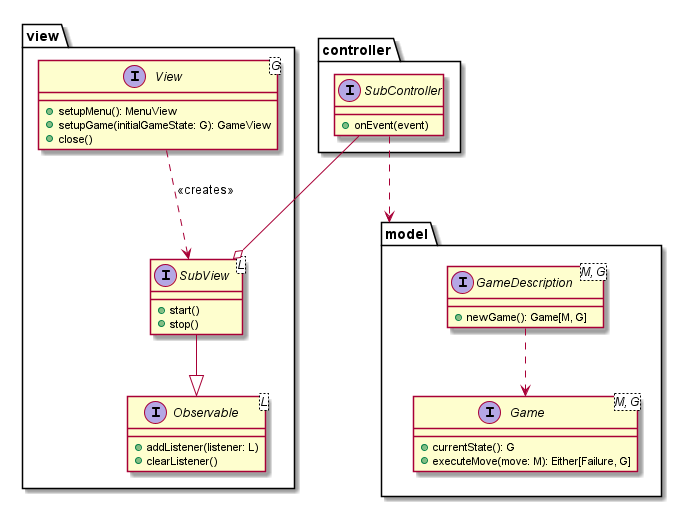
\includegraphics[width=\linewidth]{images/uml/main_class_diagram.png}
  \caption{Diagramma rappresentante le principali interfacce di model, view e controller}
  \label{fig:main_class_diagram}
\end{figure}
%
Si noti che il concetto di \texttt{SubController} presente nel diagramma non è stato effettivamente materializzato nel codice, ma è stato utilizzato per semplificare la lettura dello schema e della relativa prosa.

Ogni \texttt{SubView} specifica quale deve essere l'interfaccia del proprio tipo di listener, che viene poi implementata dal \texttt{SubController} corrispondente.
%
Quest'ultimo incapsula la logica di business della \texttt{SubView} a cui è associato e di conseguenza governa il passaggio da una \texttt{SubView} all'altra.

I listener, dopo essere stati aggiunti, vengono notificati seguendo il pattern \textbf{Observer}, in base agli eventi che accadono alla relativa \texttt{SubView}.

\subsubsection{Navigazione delle SubView}

L'architettura supporta la navigazione tra le sotto viste grazie all'interfaccia principale della View.
%
Il processo per eseguire un passaggio a una nuova \texttt{SubView} è descritto in Figura \ref{fig:view_navigation}.
%
In questo caso è stato mostrato quello relativo alla \texttt{MenuView}, ma i concetti sono generalizzabili a qualsiasi altra vista.
%
\begin{figure}
  \centering
  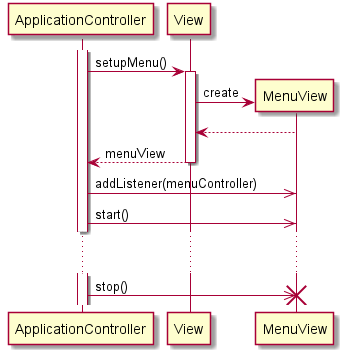
\includegraphics[width=0.6\linewidth]{images/uml/view_navigation.png}
  \caption{Interazioni necessarie per la navigazione tra SubView}
  \label{fig:view_navigation}
\end{figure}

L'interazione ha inizio generalmente da un controller, che richiede alla \texttt{View} una nuova istanza della \texttt{SubView} che vuole visualizzare.
%
In questo momento la \texttt{SubView} non è ancora visibile, per permettere al controller di registrare i listener necessari.
%
Per fare in modo che sia visibile, il controller deve richiamare il metodo \texttt{start}.

La modalità scelta per la navigazione prevede che ci sia uno \textbf{stack} di \texttt{SubView} attive in un dato momento.
%
Questo significa che ogni volta che viene aperta una nuova visualizzazione, quella precedente non viene chiusa, ma resta inattiva.
%
Quando quest'ultima viene chiusa (tramite il metodo \texttt{stop}), quella che era stata disattivata riprende il controllo e diventa la view attiva.

\newpage

\section{Design di dettaglio}\label{sec:detailed_design}

%(scelte rilevanti, pattern di progettazione, organizzazione del codice -- corredato da pochi ma efficaci diagrammi)

%Il design di dettaglio "esplode" (dettaglia) l'architettura, ma viene concettualmente prima dell'implementazione, quindi non metteteci diagrammi ultra-dettagliati estratti dal codice, quelli vanno nella parte di implementazione eventualmente.

Si affronta ora l'analisi del design di dettaglio della libreria proposta partendo dal design architetturale sopra descritto.

% ---------------------------------------------------

\subsection{Design del dominio}
% descrivere quello che è core
A fronte della \textbf{analisi del dominio} è stato individuato un nucleo di entità e funzionalità, dette \texttt{core}, necessari per lo sviluppo di giochi tramite l'utilizzo della libreria.
%
Questo \texttt{core} rispecchia quasi completamente l'analisi presentata precedentemente.
%
L'unica differenza risiede nella definizione di \texttt{Pawn} e \texttt{Tile}, che sono stati concepiti come \textbf{type members} della \texttt{BoardStructure}, e nella definizione di \texttt{Move} e \texttt{State} che sono invece stati trasformati in \textbf{generici} anziché essere definiti come interfacce vere e proprie.

Le restanti interfacce, ad eccezione di \texttt{Game}, sono state studiate per essere utilizzate come \textbf{oggetti immutabili}.
%
Questo è stato fatto anche per ridurre la rigidità, lasciando la possibilità di aggiungere certe funzionalità, per esempio, l'annullamento dell'ultima operazione fatta (Requisito \ref{req:undo}), in maniera molto semplice.
%
In questo modo è stato possibile mantenere una history degli stati passati con la certezza di non avere inconsistenze.
%
Gli oggetti immutabili inoltre aumentano la sicurezza e la leggibilità del codice.

Il \texttt{core} è la base attorno la quale sono progettati tutti gli altri moduli di questo software, presentati di seguito.

% ---------------------------------------------------

\subsection{Estensioni}

Vista la varietà di funzionalità richieste dai \textit{board game} è risultato necessario introdurre un sistema di estensioni utilizzabili opzionalmente dall'utente.

Essendo questa una libreria, non si ha conoscenza a priori dello stato del gioco e delle sue caratteristiche, perciò non è possibile fornirne una rappresentazione universale che si adatti a ogni gioco.
%
Allo stesso tempo, è anche necessario che la libreria non sia talmente generica da non offrire nessun aiuto pratico durante il suo utilizzo.

La presenza di questi molteplici requisiti ha spinto lo sviluppo del progetto in una prospettiva improntata alla modularità, che dia la possibilità allo sviluppatore finale di aggiungere agilmente funzionalità, tra quelle messe a dispozione della libreria, in maniera selettiva.
%
Questo risultato è stato raggiunto tramite il pattern delle \textbf{type class}, che permette di aggiungere funzionalità allo stato del gioco senza richiedere che questo esponga una particolare interfaccia.
%
In particolare, ogni estensione viene rappresentata come un trait generico nel tipo dello stato a cui è associato, che dichiara le funzionalità che si vogliono aggiungere allo stato.
%
Se uno sviluppatore desidera avere a disposizione una particolare funzionalità, dovrà creare una istanza di quel trait usando il proprio stato come tipo generico.
%
Infine, ogni volta che è necessaria una di quelle estensioni, è sufficiente che il codice abbia accesso all'istanza creata in precedenza.

Per convenzione, si è scelto di ospitare le dichiarazioni delle estensioni all'interno della \texttt{GameDescription}, per avere l'intera descrizione del gioco racchiusa in unico punto.

Le estensioni individuate e fornite dalla libreria sono mostrate in Figura \ref{fig:extensions}:
%
\begin{itemize}
    \item \textbf{Board state}: indica che lo stato di gioco contiene al suo interno lo stato attuale della \textit{board} (Requisito \ref{req:board_state}).
    %
    Nel design raggiunto infatti, anche la presenza di una \textit{board} è in linea teorica opzionale, nonostante sia in pratica sempre presente;
    \item \textbf{Turn state}: indica che lo stato supporta il concetto (astratto) di turno, e consente di specificare in che modo si passa da un turno a quello successivo;
    \item \textbf{Players}: indica che lo stato contiene l'elenco dei giocatori attualmente in gioco;
    \item \textbf{Game end condition}: indica che lo stato mette a disposizione una funzionalità per verificare se la partita è terminata o meno, producendo, in caso di terminazione, il risultato finale (Requisito \ref{req:end_game_cond}).
\end{itemize}
%
Si noti, che la presenza dell'associazione è sempre opzionale nel lato dell'estensione, questo per mettere in evidenza che un gioco non è obbligato ad implementare tale estensione.
%
\begin{figure}
    \centering
    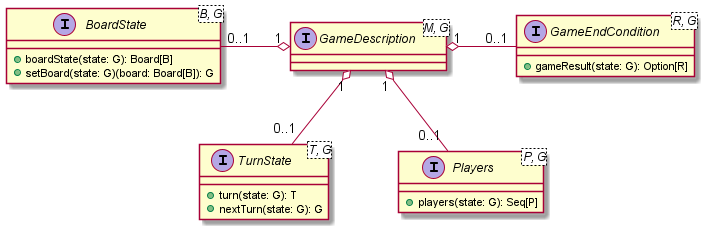
\includegraphics[width=\linewidth]{images/uml/extensions.png}
    \caption{Diagramma delle classi per le estensioni dello stato}
    \label{fig:extensions}
\end{figure}

% ---------------------------------------------------

\subsection{RuleSet e Dsl}\label{sec:dsl_design}

Si analizza ora il design di dettaglio relativo al \texttt{RuleSet} e al suo \textbf{DSL}.

Il \texttt{RuleSet} idendifica l'insieme delle regole che definiscono se, in un determinato stato, una \textit{move} è valida e in quale modo questa modifichi lo stato del gioco al momento della sua esecuzione (Requisiti \ref{req:dsl}).
%
La modalità con cui viene abilitato l'utilizzo del DSL, all'interno della definizione del proprio \texttt{RuleSet}, consiste nel dichiarare una classe (o un oggetto) che estenda dal trait \texttt{RuleSet} e aggiungere il trait \texttt{RuleSetBuilder} come mixin.
%
In questo modo, lo sviluppatore ha a disposizione una sintassi e un insieme di parole chiave definite dalla libreria.
%
La modalità scelta introduce, per il team, il problema di come organizzare le dichiarazioni delle parole chiave per fare in modo che la soluzione sia modulare e scalabile.
%
Il DSL, per questo motivo, è stato suddiviso in diverse componenti per mantenere un alto livello di modularità.
%
In seguito ciascuna componente è stata unificata, tramite l'utilizzo dell'ereditarietà multipla tramite mixin, in un unico trait (\texttt{RuleSetBuilder}) per consentire all'utente di abilitare l'intera sintassi con una sola dichiarazione.

Le componenti individuate sono descritte nei paragrafi seguenti.

\paragraph{MovesGeneration e MovesExecution}
Rappresentano il punto di collegamento tra il DSL e il \texttt{RuleSet}, poichè accumulano le varie regole scritte all'interno del sorgente in un unico punto e lo rendono disponibile per essere utilizzato come implementazione dell'interfaccia del \texttt{RuleSet}.

\subparagraph{Generators}
Un \texttt{Generator} rappresenta l'astrazione di base utilizzata per la generazione delle mosse ed è costituito da una funzione che, partendo da uno stato di gioco, genera un certo insieme di mosse valide (Requisito \ref{req:generator}).
%
Tramite la componente \texttt{Generators} viene fornita all'utente la sintassi per la creazione dei generatori più comuni.

\subparagraph{Actions}
Come la \texttt{MovesGeneration} è fondata sul concetto di \texttt{Generator} come astrazione base, così la componente \texttt{MovesExecution} è fondata sul concetto di \texttt{Action}.
%
Una \texttt{Action} è rappresentata da una funzione che, a partire da uno stato, restituisce un nuovo stato.
%
Le \texttt{Action} sono le azioni che saranno poi utilizzate per modificare lo stato come da requisito \ref{req:action}

Anche in questo caso, la componente \texttt{Actions} fornisce la sintassi per poter utilizzare le azioni più frequentemente impiegate nei giochi da tavolo.

\paragraph{Chainables e Modifiers}
Una volta forniti i mattoncini di base per la generazione e l'esecuzione delle mosse (rispettivamente \texttt{Generator} e \texttt{Action}), vengono forniti all'utente della libreria dei costrutti che consentono di combinare in diversi modi queste astrazioni.
%
Lo scopo è quello di permettere la creazione di azioni composite o di generatori più complessi, evitando di dover reinventare costantemente la ruota e riutilizzando il più possibile i meccanismi già implementati.

La soluzione fornita dalla libreria prevede la possibilità di \textbf{concatenare} tra di loro i meccanismi di base producendo nuove azioni o generatori, a loro volta combinabili.
%
Questa funzionalità è abilitata dalla type class \texttt{Chainable} (Figura \ref{fig:chainables}), che rappresenta una trasformazione \textbf{concatenabile} a un altra trasformazione dello stesso tipo.
%
\begin{figure}
    \centering
    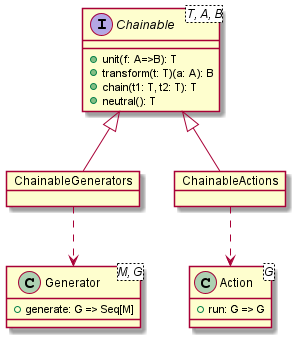
\includegraphics[width=0.5\linewidth]{images/uml/chainables.png}
    \caption{Diagramma delle classi contentente la struttura dei Chainable}
    \label{fig:chainables}
\end{figure}

Un tipo \texttt{Chainable} deve definire il modo in cui viene prodotto il risultato della concatenazione e deve inoltre definire il proprio \textbf{elemento neutro} (ovvero quello la cui concatenazione con qualsiasi altro elemento produce l'elemento stesso).
%
In questo possono essere considerati come dei \textbf{Monoidi}.
%
In più un \texttt{Chainable} è anche una trasformazione da un tipo \texttt{A} a un tipo \texttt{B}, entrambi definiti dall'istanza stessa di \texttt{Chainable}.
%
Il trait \texttt{Chainable} richiede quindi di definire un operatore \texttt{unit} che produce una trasformazione \texttt{T} a partire da una semplice funzione e un operatore \texttt{transform} che applica la trasformazione a un elemento.

Questa definizione consente di sfruttare il concetto di \texttt{Chainable} per permettere a generatori ed azioni di essere utilizzati all'interno dei \textbf{costrutti iterativi e condizionali} (\texttt{Modifiers}) messi a disposizione dal DSL della libreria.
%
I dettagli implementativi di come ciò avviene saranno descritti nella Sezione \ref{sec:dsl_syntax}.

\paragraph{Features}
Essendo il \texttt{RuleSet} definito a livello intensionale, è necessario avere un meccanismo per rappresentare le proprietà dello stato anche non avendo a disposizione una particolare istanza dello stesso.
%
Questa problematica è risolta dal concetto di \texttt{Feature}, ovvero una funzione che estrae dallo stato una sua proprietà.

La componente \texttt{Features} dichiara un insieme di \texttt{Feature} comunemente utilizzate.

% ---------------------------------------------------

\subsection{Interazione}

Le funzionalità abilitanti l'interazione con i giocatori sono state incapsulate totalmente nel modulo \texttt{interaction}, che comprende \texttt{view} e \texttt{controller}, con un interfacciamento verso il \texttt{model}.

Un gioco completo sviluppato con la libreria prevede due viste principali:
\begin{itemize}
    \item \textit{Menu}: il punto di ingresso dell'applicazione dove poter selezionare opzioni come giocare una nuova partita oppure uscire dal programma;
    \item \textit{Game}: una partita in corso.
\end{itemize}
%
Ciascuna di queste è composta da una specifica coppia di \texttt{SubView} e \texttt{SubController}.

\subsubsection{View}

La \texttt{View} principale è in grado di creare e inizializzare le \texttt{SubView} esponendo un metodo per ritornare ognuna di esse, semplificando la navigazione fra le \texttt{SubView}.

\paragraph{Menu view} 
È il componente per gestire tutto ciò che è precedente o successivo al \textit{Game} (es. avvio di un \textit{Game}, chiusura dell'applicazione).
%
Il \texttt{MenuView} permette tramite un'apposita UI di scegliere come procedere tra le varie opzioni.

\paragraph{Game view}

È la \texttt{SubView} responsabile della rappresentazione del gioco nel suo stato attuale e di gestire l'interazione con l'utente che inserisce dei comandi.

\subparagraph{Renderer}
Per effettuare il display dello stato del gioco, la \texttt{GameView} utilizza un certo insieme di \texttt{Renderer}, che sono responsabili della visualizzazione di uno specifico sottoinsieme delle informazioni da mostrare (Requisito \ref{req:renderers_parameters}).
%
Questa scelta è stata effettuata in quanto giochi diversi hanno proprietà diverse che devono essere mostrate all'utente, ed è necessario separare le diverse visualizzazioni al fine di renderle riutilizzabili e seguire il principio di singola responsabilità.
%
In particolare, quando le proprietà da visualizzare corrispondono alle \texttt{extension} è possibile utilizzare un \texttt{Renderer} comune a tutti i giochi con quella specifica estensione.
%
Richiamando l'aggiornamento di tutti i \texttt{Renderer} la \texttt{GameView} è in grado di mostare tutte le caratteristiche dello stato attuale del \textit{Game}.

\subparagraph{Event}
Ogni volta che un utente interagisce con la \texttt{GameView} inserendo dei comandi, quest'ultima genera degli \texttt{Event} che vengono ascoltati dal \texttt{GameController}.
%
Questo è a conoscenza del modo in cui convertire questi eventi in mosse da eseguire sullo stato o in altre azioni particolari.

% ---------------------------------------------------

\subsubsection{Controller}
I controller presentano una dipendenza dalle view in quanto devono chiamare i metodi della specifica \texttt{SubView} per fornire il feedback appropriato rispetto all'interazione intrapresa dal giocatore.
%
L'\texttt{ApplicationController} è responsabile di gestire la \texttt{View} principale, scegliendo quale \texttt{SubView} mostrare e aggiungendovi i \textbf{listener} relativi.

\paragraph{Menu controller}
Presenta le funzionalità per gestire l'avvio di una partita e la terminazione dell'applicazione.
%
Questo controller è una prima interfaccia con il \textbf{model}, che nel caso di avvio di una partita utilizza la \texttt{GameDescription} per la generazione di un nuovo \texttt{Game}.
%
Successivamente prepara la GameView con i parametri relativi, aggiunge un nuovo \texttt{GameController} come listener e passa alla nuova vista.

\paragraph{Game controller}
%
Come descritto in precedenza, il \texttt{GameController} gestisce gli \texttt{Event} che gli vengono notificati, presentando un comportamento diverso in base alla situazione (Requisito \ref{req:events}):
%
\begin{itemize}
    \item Se l'evento è \texttt{Quit} allora termina la \texttt{GameView}.
    \item Se l'evento è \texttt{Undo} allora annulla l'ultima mossa eseguita.
    \item Se l'evento è \texttt{Clear} allora viene svuotata l'attuale coda degli eventi.
    \item In tutti gli altri casi, gli eventi vengono accodati fino a che non vengono riconosciuti come mossa.
\end{itemize}
%
Quando viene riconosciuta una mossa, la coda degli eventi viene svuotata e la mossa viene eseguita (tramite \texttt{executeMove}) sull'istanza corrente del \texttt{Game}, producendo due possibilità:
\begin{itemize}
    \item se la mossa è valida per lo stato attuale del gioco, viene eseguita e la chiamata restituisce il nuovo stato prodotto;
    \item se la mossa non è valida o se viene lanciata un'eccezione durante l'esecuzione, viene restituita una failure che descrive cosa non ha funzionato.
\end{itemize}
%
In entrambi i casi il risultato della chiamata viene comunicato alla \texttt{GameView} chiamando un metodo tra \texttt{moveAccepted} o \texttt{moveRejected}.
%
La Figura \ref{fig:gui_sequence} mostra più schematicamente come avviene questa interazione.
\begin{figure}
  \centering
  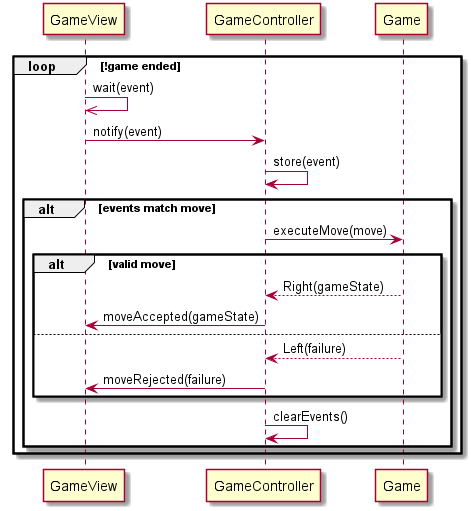
\includegraphics[width=\linewidth]{images/uml/gui_sequence.png}
  \caption{Diagramma di sequenza rappresentante le interazioni in un game tra model, view e controller}
  \label{fig:gui_sequence}
\end{figure}



\newpage

\section{Implementazione}

La seguente sezione va ad analizzare quelli che sono gli aspetti e le decisioni implementative che caratterizzano il codice.
%
Si riportano solo i casi degni di nota e si lascia il resto al codice e alla documentazione su di esso, che sono stati pensati per essere autoesplicativi e semplici da comprendere per un utilizzatore della libreria.

% ---------------------------------------------------

\subsection{Passaggio implicito delle type class}

Come anticipato nella Sezione \ref{sec:detailed_design}, il meccanismo delle type class è stato sfruttato molto frequentemente.
%
Al fine di massimizzare la pulizia e la leggibilità del codice, si è deciso di utilizzare il passaggio implicito dei parametri per evitare di dover comunicare esplicitamente le istanze delle type class.

% ---------------------------------------------------

\subsection{Sintassi del DSL}\label{sec:dsl_syntax}

Il DSL è stato scritto in maniera quanto più auto-esplicativa possibile, in modo da mettere l'utente della libreria nella condizione di dover fare il minor sforzo possibile per la scrittura delle regole di un gioco.
%
Questo ci ha portato alla scrittura di un DSL molto simile (ove possibile) al linguaggio naturale e che richiede una conoscenza estremamente limitata del linguaggio Scala.

Per ottenere questo risultato è stato necessario sfruttare alcune funzionalità offerte da Scala:
\begin{itemize}
  \item \textbf{metodi come operatori infissi}, che richiedono quindi che un metodo sia preceduto e seguito da un oggetto;
  \item \textbf{conversioni implicite}, per aggiungere metodi a tipi già esistenti o per adattare oggetti in maniera trasparente;
  \item \textbf{uso delle parentesi graffe al posto delle parentesi tonde}, per avere una strutturazione più familiare nel caso di nesting dei costrutti.
\end{itemize}

I meccanismi citati, specialmente il primo, richiedono spesso l'adattamento della struttra sintattica delle frasi, scritte in linguaggio naturale, per fare in modo che sia supportata a livello sintattico anche da Scala.
%
In particolare si è cercato di adattare il più possibile le frasi del DSL, per fare in modo che la struttura potesse essere ricondotta a sequenze del tipo \texttt{object method object method object ...}, in modo da evitare la presenza di parentesi.

Nel Listato \ref{lst:dsl_example} è mostrato uno snippet di codice che mostra a grandi linee le modalità con cui i meccanismi di scala sono stati adottati nella scrittura del costrutto iterativo.
%
\lstinputlisting[language=scala, caption={Dichiarazione della sintassi di iterazione e esempio di utilizzo}, label=lst:dsl_example]{code/dsl.scala}
%
Un'istruzione di iterazione parte dalla parola chiave \texttt{iterating} (Requisito \ref{req:iterating}), ovvero un oggetto il cui unico metodo è \texttt{over}.
%
Questo metodo accetta una \texttt{Feature} che estrae dallo stato un \texttt{Traversable[F]} su cui deve essere eseguita l'iterazione.
%
Come anticipato nella Sezione \ref{sec:dsl_design}, è necessario usare una \texttt{Feature} poichè le regole vengono definite a livello intensionale, quindi non si ha accesso diretto allo stato.

Il metodo \texttt{over} restituisce un nuovo oggetto di tipo \texttt{Iteration[F]}, che a sua volta contiene un unico metodo \texttt{as} al quale deve essere passata la funzione di iterazione.
%
Questa è una funzione che associa ad ogni elemento estratto dallo stato un nuovo oggetto di tipo \texttt{T} generico.
%
Per fare in modo che l'iterazione sia possibile, è necessario anche che sia implicitamente definita un'istanza di \texttt{Chainable}, per stabilire in che modo concatenare le \texttt{T} restituite dalle singole iterazioni e quale deve essere il valore di partenza per l'accumulazione.

Infine viene mostrato un esempio di utilizzo del costrutto di iterazione su una proprietà \texttt{Traversable} dello stato.
%
L'esempio utilizza il metodo \texttt{generate} fornito dalla libreria, che restituisce un oggetto di tipo \texttt{Generator}, per cui la libreria fornisce già un'istanza di \texttt{Chainable}.

% ---------------------------------------------------

\subsection{Cli}
%
Data l'infrastruttura di gestione dell'interazione con il giocatore, un utente della libreria può scegliere se scrivere una propria implementazione dell'interfaccia grafica (Requisito \ref{req:custom_view} oppure se avvalersi dell'interfaccia a riga di comando fornita dalla libreria (Requisito \ref{req:cli}).
%
Questa opzione è compatibile solamente con i giochi aventi una \textit{Board} \textbf{rettangolare}, per tutti gli altri è necessario fornire un'implementazione alternativa.

L'interfaccia a riga di comando è generata a partire dalle caratteristiche del gioco e dai \texttt{Renderer} associati, seguendo così un approccio standardizzato per associare a diverse \textbf{estensioni} del gioco una specifica rappresentazione in maniera automatica.
%
Ciò consente di avere una visualizzazione semplice del gioco scritto usando la libreria, con il minimo sforzo da parte dell'utente, che ha però la possibilità di personalizzare la grafica fornendo una serie di parametri oppure nuove implementazioni dei singoli componenti per i quali desidera un aspetto diverso.
%
In particolare gli aspetti personalizzabili per il \texttt{BoardRenderer} sono:
\begin{itemize}
  \item Rappresentazione degli indici delle colonne;
  \item Rappresentazione degli indici delle righe;
  \item Separatore degli elementi grafici;
  \item Terminazione riga;
  \item Rappresentazione dei \textit{Tile} vuoti;
  \item Rappresentazione dei diversi \textit{Pawn}.
\end{itemize}
%
Ognuno di questi parametri ha un valore di default, seguendo il principio della \textbf{convenzione} prima della \textbf{personalizzazione} in modo da snellire il processo di preparazione dell'interfaccia da parte dell'utente qualora le impostazioni base fossero sufficienti.
%
Infine, i \texttt{Renderer} rimanenti non sono parametrici in quanto sufficientemente semplici da poter essere completamente sostituiti in maniera rapida da nuove implementazioni.

% ---------------------------------------------------

\subsection{Configurazione dell'app: GameSetup}

La configurazione degli elementi che gestiscono l'interazione tra un giocatore umano e l'applicazione finale richiede svariati passaggi.
%
È necessario che lo sviluppatore configuri correttamente i parametri di rendering, la comunicazione tra view e controller e altri dettagli spesso dipendenti l'uno con l'altro.

Per porre rimedio a questo problema e per fornire un singolo punto di configurazione, è stato creato un piccolo modulo di utility -- il \texttt{GameSetup} -- che ha l'obiettivo di aiutare lo sviluppatore fornendo uno scheletro della configurazione, implementato con valori di default considerati standard.
%
Questo modulo consente a chi utilizza la libreria di fornire la propria configurazione personalizzata facendo override dei metodi presenti nel \texttt{GameSetup} in stile \textbf{template method}.

La libreria supporta al momento una configurazione dettagliata solo per l'interfaccia testuale (estendendo il trait \texttt{CliGameSetup}), ed in particolar modo aiuta lo sviluppatore nel caso venga utilizzata una board di tipo rettangolare (aggiungendo il mixin \texttt{RectangularBoardSetup}).
%
Le principali funzionalità che sono state fornite sono:
%
\begin{itemize}
  \item Scelta dei renderer che dovranno essere utilizzati a partire da un \textbf{builder}, per poter scegliere dinamicamente cosa disegnare;
  \item Configurazione del parsing dei comandi a partire da un \textbf{builder}, per aggiungere dinamicamente comandi con sintassi arbitrarie;
  \item Sintassi semplificata per i metodi di entrambi i builder, che sono internamente implementati come template method che richiamano i metodi potenzialmente sovra\-scrivibili dallo sviluppatore stesso.
\end{itemize}

Una volta scritta la propria configurazione nel \texttt{GameSetup}, è possibile avviare l'ap\-pli\-ca\-zione chiamando \texttt{AppRunner.run} fornendo la propria istanza di \texttt{GameSetup}, che viene generalmente chiamato dall'interno dell'entry point dell'app.

% ---------------------------------------------------

\subsection{Giochi}
Oltre alla libreria stessa sono stati sviluppati alcuni giochi per fungere da esempi per gli utenti e dimostrare l'utilizzo delle funzionalità proposte.
%
I giochi realizzati sono i quattro descritti nei requisiti, e sono stati scelti sia per le loro caratteristiche che per fornire diversi livelli di complessità implementativa.

Si fa ora una breve analisi della struttura di \textit{Connect four} come esempio cardine.
%
Questo gioco è stato scelto poiché la sua complessità è tale da mostrare le potenzialità della libreria senza richiedere un'analisi troppo complicata.
%
Per scrivere un gioco si parte dalla defizionione di quelli che sono gli aspetti del modello, ovvero: 
\begin{itemize}
  \item il trait \texttt{ConnectFourPawn} che rapresenta i \textit{pawn};
  \item la \textit{move} \texttt{Put} che indica l'inserimento di una pedina all'interno di una colonna;
  \item \texttt{ConnectFourBoard} una board rettangolare;
  \item \texttt{ConnectFourState} che racchiude il riferimento alla \textit{board} e al \textit{player} corrente.
\end{itemize}
%
Definiti quelli che sono gli aspetti del modello si passa alla definizione del \textit{rule set}.
%
Questo estende da \texttt{RuleSet} ed utilizza il mixin \texttt{RuleSetBuilder} per abilitare le funzionalità del DSL offerte dalla libreria.
%

\lstinputlisting[language=scala, caption={Connect four rule set}, label=lst:connect4_rule_set_example]{code/ConnectFourRuleSet.scala}

%
Come è possibile vedere dal codice Listato \ref{lst:connect4_rule_set_example} si definisce una apposita \texttt{Feature} per estrarre dallo stato la prima \textit{tile} libera di una colonna.
%
Si usa quindi questa \texttt{Feature} appena definita per specificare in quale modo l'azione \texttt{Put} sopra definita agisca sullo stato, ovvero, (traducendo quello che in inglese è presente nel codice) piazzando il turno corrente sulla prima cella libera della colonna x.
%
Si definisce poi quando il turno deve cambiare, ovvero dopo ogni mossa.
%
Infine, si specifica che la mossa \texttt{Put} è valida e deve essere generata per ogni colonna in cui la \textit{tile} che si trova in cima non è occupata.

Ora è necessario creare una entità che estenda da \texttt{GameDescription} dentro la quale definire tutte le caratteristiche che deve avere il gioco.
%
\lstinputlisting[language=scala, caption={Connect four game description}, label=lst:connect4_game_description]{code/ConnectFourGDescr.scala}
%
In particolare, si definiscono:
\begin{itemize}
  \item lo stato iniziale;
  \item il \textit{rule set};
  \item i player;
  \item i turni associandoli ai player, in questo modo \texttt{currentTurn} rapresenta sia il turno che il player;
  \item le \textit{endCondition} che definiscono le condizioni di terminazione di una partita.
\end{itemize}
%
Si nota, nel Listato \ref{lst:connect4_game_description}, che i valori sono definiti in modo implicito per semplificare l'utilizzo del \textit{rule set} e del resto della libreria.

\lstinputlisting[language=scala, caption={Connect four main e game setUp}, label=lst:connect4_main]{code/ConnectFourMain.scala}
%
Infine, come mostrato nel Listato \ref{lst:connect4_main}, definendo un \texttt{ConnectFourSetUp} che estende da \texttt{CliGameSetUp} si ottiene senza alcuno sforzo una rappresentazione testuale del gioco e la possibilità di eseguire il gioco appena scritto.

% ---------------------------------------------------

\subsection{Testing}
I test effettuati sul codice sviluppato hanno lo scopo principalmente di garantire la qualità del codice, di favorire il cambiamento ed infine di documentazione del software sviluppato, seguendo la \textbf{quality school} e la \textbf{agile school} come filosofie di riferimento.
%
Avendo approcciato il progetto con la metodologia \textbf{TDD} la maggior parte del codice risulta avere degli unit test che coprono le singole funzionalità.
%
Ci sono alcune eccezioni, ad esempio l'interfaccia testuale risulta essere poco coperta dai test a causa della necessità di acquisire input da tastiera e la scarsa utilità di testare i risultati di stampe a video.
%
La copertura risulta invece molto alta nel \texttt{model}, arrivando ad avere il 100\% di coverage per il \texttt{core}.
%
Oltre agli \textbf{unit test} utilizzati per l'approccio TDD e sviluppati prima del codice stesso, sono presenti anche degli \textbf{integration test}, aggiunti una volta terminato lo sviluppo del codice di una singola unità per assicurare la corretta interazione con le altre.
%
Infine, i \textbf{system test} sono stati effettuati nei giochi d'esempio, che forniscono un ambiente articolato e completo dove poter testare l'interazione fra i diversi moduli del sistema.

\subsubsection{Test doubles}
Ove possibile sono stati effettuati test di tipo funzionale e \textbf{blackboxed}, mentre dove è risultato necessario sono stati effettuati dei test strutturali \textbf{whiteboxed}.
%
Entrambi le casistiche hanno visto un impiego frequente dei \textbf{test doubles} sfruttando la libreria \textbf{scalamock} per rimuovere le dipendenze dagli unit test o per verificare il comportamento interno di un componente nel caso di test whitebox.

\subsubsection{Stile dei test}
Lo stile adottato è stato \textbf{FlatSpec} nella quasi totalità dei casi, in quanto il più adatto agli unit test e semplice sia da consultare che da modificare, a favore di uno sviluppo agile del software a fronte di cambiamenti nei requisiti o nella loro comprensione da parte del team.

% ---------------------------------------------------

\subsection{Divisione del lavoro}
%parti comuni:
% - core
% - extension
% - divisione in due sottogruppi per la gestione delle due macro-componenti del progetto
% -- Comuni: RuleSet, DSL, Features
La divisione del lavoro del team si può suddividere in tre stadi:
%
\begin{inparaenum}[1)]
\item Inizialmente il gruppo ha affrontato l'analisi del dominio e l'analisi architetturale dell'intero sistema in completa collaborazione, tramite meeting intensi nei quali si è cercato di delineare quelli fossero gli obiettivi del team nel breve e lungo periodo.
%
\item Una volta stabilito quello che è il design architetturarale del sistema si è scelto di dividere il team in due sotto-team di due persone ciascuno.
%
Il primo gruppo è quello formato da Dente ed Evangelisti al quale è stato assegnato il compito di lavorare sul \textit{rule set} e sul \textit{DSL} relativo.
%
Il secondo gruppo formato da Magnani e Nemati si è occupato principalemente della parte di interaction.
%
\item In fine, all'interno di ogni gruppo, dopo aver effettuato un'attenta analisi in dettaglio delle sezioni di interesse, si è suddiviso il lavoro per singoli membri.
\end{inparaenum}

Le divisioni del lavoro svolte sono state sempre ben documentate nel corso dello svolgimento del progetto ma è da tenere in considerazione che la stretta collaborazione e il continuo ciclo di daily scrum ha fatto in modo che tutti i membri del gruppo fossero sempre tenuti al corrente dell'andamento del progetto.
%
Si sottolinea che buona parte del codice è stata scritta in \textbf{pair programming} per massimizzare la qualità del codice e ridurre il tempo relativo alla revisione del codice.

\subsubsection{Dente Francesco}

La porzione principale del progetto di cui mi sono occupato è stata la scrittura e la progettazione del DSL per la definizione del \textit{rule set}, svolta in collaborazione con Evangelisti.
%
In particolare, nonostante gran parte del lavoro sia stata portata avanti cooperativamente, ho dato un contributo particolare nella scrittura del codice relativo alla generazione delle mosse e all'utilizzo del concetto di Chainable all'interno dei costrutti iterativi e condizionali.

Per quanto riguarda invece la parte core della libreria, mi sono occupato dell'in\-tro\-du\-zione delle type class per implementare le estensioni dello stato, nonostante queste siano state poi aggiornate con le successive iterazioni in maniera cooperativa da tutti i membri del gruppo.

Un'altra area su cui mi sono concentrato è stata l'implementazione delle astrazioni di GameSetup e in generale della gestione della fase di configurazione e avvio dell'ap\-pli\-ca\-zione.

Infine, mi sono occupato dello sviluppo e del testing del gioco d'esempio Othello, che è stato implementato una volta terminata la scrittura del codice della libreria in sè.

\subsubsection{Evangelisti Davide}
% dsl in comune con Dente, RuleSet (con particolare attenzione alla move execution e le Action), PutInPutOut Revisited, 'after each move', RuleSetBuilder
% RuleSetBuilder
% MovesExecution
Mi sono occupato principalemente della scrittura del \textit{rule set} assieme al collega Dente con il quale ho affrontato l'analisi del problema e la progettazione di massima del DSL.
%
La parte, del \textit{rule set} alla quale mi sono dedicato maggiormente è stata quella relativa all'esecuzione delle \textit{move} e al relativo DSL, che permette all'utente della libreria di scrivere facilmente in quale modo lo stato del gioco viene modificato da un'azione.
%
Nello specifico mi sono occupato del trait \texttt{MovesExecution}, nel quale, tramite le funzionalità offerte da Scala, ho costruito la parte di DSL relativa all'esecuzione delle \textit{move}.
%
Grazie alle conversioni implicite sono riuscito a rendere la \texttt{MovesExecution} indipendente dal sistema delle \texttt{Actions} e allo stesso tempo queste ultime si integrano perfettamente all'interno del sistema di creazione delle \textit{move}.

Per quanto riguarda il \texttt{RuleSet} e il \texttt{RuleSetBuiledr} ho scelto di dividere questi due aspetti in modo da rendere il \texttt{RuleSet} indipendente dal modo in cui questo è generato.
%
Così facendo do la possibilità a chi utilizza la libreria di scegliere se utilizzare il DSL oppure approciarsi alla generazione e all'esecuzione delle mosse in un modo diverso.

Oltre alla parte relativa al \textit{rule set} mi sono occupato anche della \textit{Board} e della sua scrittura.
%
In questo particolare frangente non sono presenti tecniche di programmazione avanzate se non l'immutabilità della \textit{Board} stessa.
%
Si è scelto di mantenere la \textit{Board} immutabile in vista di modifiche future e di funzionalità aggiuntive della libreria, questa scelta si è dimostrata corretta in quanto durante la scrittura della funzionalità opzionale di \textbf{undo}, ovvero la possibilità di tornare allo stato precedente, la presenza di un oggetto immutabile semplifica enormemente il lavoro.

Oltre a questo mi sono occupato dello sviluppo e del mantenimento del primo gioco sviluppato dal gruppo, ovvero, PutInPutOut.

\subsubsection{Magnani Simone}
% interaction in comune con Nemati. In singolo:
Dopo lo sviluppo delle parti comuni e la divisione in sottogruppi, insieme a Nemati, abbiamo lavorato allo sviluppo di tutto ciò che riguarda l'interazione con l'utente.
% View - GameView
In particolare, occupandomi della \texttt{View} ho cercato di rendere la generazione di ogni componente il più lontano possibile dal \texttt{model}, tanto che per giochi con \textit{Board} rettangolari esiste un'implementazione automatica della visualizzazione ed interazione.
% renderer
Ho sviluppato i \texttt{Renderer} in modo da comporre la \texttt{GameView}, ma incapsulando l'obiettivo specifico di ogni \texttt{Renderer}.
%
Questo ha reso la \texttt{GameView} indipendente dalle varie \texttt{extension} di ogni particolare gioco permettendo la generazione automatica della stessa.
%
\'E importante anche menzionare il \texttt{CliBoardRenderer}, che tramite la configurazione dei \texttt{Converter} nel \texttt{CliGameSetup}, rende personalizzabile la visualizzazione della \textit{Board} in relazione alla selezione dei \textit{Tile}.
% Connect4
Infine mi sono occupato del testing e dell'implementazione di \textbf{Connect Four}, il che mi ha portato a realizzare delle \texttt{apply} di utility per le \texttt{extension}.

\subsubsection{Nemati Shapour}
% interaction in comune con Magnani.
In seguito al lavoro comune iniziale, la parte a cui ho contribuito maggiormente è stata quella di interazione utente, assieme a Magnani.
%In singolo:
% Controller
Personalmente ho lavorato al \textbf{controller}, in particolare al \textbf{GameController} ed alla sua interazione con il \textbf{Model}, gestendo l'unico punto di contatto fra questi, anche se successivamente la parte di gestione degli errori è stata spostata dal controller al model.
% Event
Per gestire l'interazione fra \textbf{controller} e \textbf{view} ho gestito lo sviluppo degli \texttt{Event} come elemento base di interazione che possa essere indipendente dal tipo di view e sempre costante per il controller.
% Input parser
Nel lavorare a stretto contatto con la parte di \textbf{cli} ho poi sviluppato l'\textbf{Input Parser} che gestisce la conversione dal testo digitato dall'utente agli \texttt{Event} gestibili dal controller, anche se successivamente questa parte è stata riadattata da Dente per semplificarne l'utilizzo nel caso in cui lo sviluppatore non volesse ricorrere alle espressioni regolari per definire il proprio mapping fra stringhe ed eventi.

% Rectangular Board
Per quanto riguarda il mio contributo ai giochi ho espanso le funzionalità delle \textit{board} rettangolari in modo da fornirne le diagonali all'utente, che in svariati giochi potrebbe voler conoscere lo stato di una o più diagonali.

% Tic-Tac-Toe
Infine ho sviluppato il gioco Tic-Tac-Toe, utile campo di prova per la generazione automatica della \textbf{cli} oltre che delle estensioni.
\newpage

\section{Restrospettiva}

%(descrizione finale dettagliata dell'andamento dello sviluppo, del backlog, delle iterazioni; commenti finali)

%Si noti che la retrospettiva è l'unica sezione che può citare aneddoti di cosa è successo in itinere, mentre le altre sezioni fotografino il risultato finale. Se gli studenti decideranno (come auspicato) di utilizzare un product backlog e/o dei backlog delle varie iterazioni/sprint, è opportuno che questi siano file testuali tenuti in versione in una cartella "process", così che sia ri-verificabile a posteriori la storia del progetto.

\subsection{Sprint 1}
Il primo sprint è stato principalmente incentrato sul setup del progetto, l'analisi del problema e la creazione delle interfacce core della libreria, questo ha portato a meeting molto frequenti e prolungati durante la giornata.
\paragraph{Svolgimento e sviluppo dello sprint}
Sono stati inizializzati i tool inerenti al processo di sviluppo, in particolare:
\begin{itemize}
   \item \textbf{SBT} per la gestione delle dipendenze e delle build;
   \item \textbf{Travis CI} per il testing automatico e la Continous Integration.
\end{itemize}
Si è ritenuto necessario sin da subito creare convenzioni comuni riguardo i termini, la documentazione e la scrittura di codice, ad esempio l'uso di un glossario comune.
%
Dopo una prima parte di Design, sono stati scritti i test e le relative interfacce necessarie alla creazione del gioco PutInPutOut; infine sono stati creati i test del gioco tramite i requisiti specificati ed è stato implementato il gioco.
\paragraph{Considerazioni finali}
Lo sprint non ha sollevato particolari problemi ed è terminato nei tempi previsti.

Una possibile prosecuzione prevede:
\begin{itemize}
  \item la possibilità di avere dei \textbf{turni} e dei giocatori all'interno della partita;
  \item un'interfaccia più facilmente utilizzabile per l'utente della libreria;
  \item l'implementazione del gioco \textbf{Tic-Tac-Toe}.
\end{itemize}

\subsection{Sprint 2}
Il secondo sprint è stato principalmente incentrato sull'estensione delle funzionalità core della libreria, lo sviluppo di utility comunemente adottate dai giochi target della libreria e la creazione del gioco Tic-Tac-Toe.
\paragraph{Svolgimento e sviluppo dello sprint}
Lo sviluppo della libreria è stato parallelizzato alla creazione di Tic-Tac-Toe.
%
Alcuni dei requisiti di Tic-Tac-Toe sono stati resi più generali al fine di integrarli nella libreria: in particolare la necessità di avere dei \textit{player}, un \textit{game flow} basato su turni e su \textit{game ending conditions}.
\paragraph{Considerazioni finali}
Durante lo sprint si sono riscontrati problemi con l'utilizzo di \textbf{ScalaMock} e, data la complessità del progetto, il team si è trovato a lavorare sulle stesse funzionalità, portando a una minore parallelizzazione dei task e, di conseguenza, a un minor rigore nel processo di sviluppo.

Una possibile prosecuzione prevede:
\begin{itemize}
  \item un'interfaccia più facilmente utilizzabile per l'utente della libreria;
  \item l'implementazione di una interfaccia visuale del gioco \textbf{Tic-Tac-Toe}.
\end{itemize}

\subsection{Sprint 3}
Il terzo sprint aveva inizialmente lo scopo di sviluppare un primo DSL ed un'interfaccia utente testuale, ma a causa di rigidità del codice precedente è stato necessario operare un \textbf{refactor} su una grande porzione di codice, e come risultato non è stato possibile raggiungere gli obiettivi prefissati.
\paragraph{Considerazioni finali}
Dal punto di vista del processo di sviluppo la metodologia \textbf{Scrum} non è stata seguita in toto, in particolare i Daily Scrum non sempre hanno avuto luogo seguendo gli step prestabiliti, ma si è proceduto in gruppo a lavorare sul codice da rifattorizzare.

Una possibile prosecuzione prevede il completamento dei Task ancora aperti a cui va ad aggiungersi lo sviluppo del gioco \textbf{Connect Four}.

\subsection{Sprint 4}
Il quarto Sprint ha raggiunto con successo gli obiettivi posti: lo sviluppo di un primo DSL, di un'interfaccia utente testuale, e del gioco \textbf{Connect Four}.
\paragraph{Considerazioni finali}
La metodologia \textbf{Scrum} è stata applicata efficacemente, cor\-reg\-gendo gli errori fatti negli Sprint precedenti.
%
Una possibile miglioria riguardante gli strumenti a supporto del processo di sviluppo è quella di individuare dei \textbf{Task} a grana più fine ed inserirli in \textbf{Trello}, al fine di guadagnare in autonomia dei membri del team, e di ottenere una maggiore chiarezza su quali funzionalità siano già pronte, quali in sviluppo, e quali totalmente assenti.

Una possibile prosecuzione prevede di migliorarela qualità del codice, ed aggiungere alcune funzionalità in più per quanto riguarda il DSL e l'interfaccia testuale.

\subsection{Sprint 5}
Il quinto Sprint ha portato gli incrementi attesi, fornendo un DSL più potente ed una view più dinamica.
\paragraph{Considerazioni finali}
A causa di impegni personali di alcuni membri del team non sempre si sono tenuti i \textbf{Daily Scrum} con la presenza di tutto il team, ma oltre questo piccolo inconveniente non si riscontrano altre problematiche di processo.

Una possibile prosecuzione prevede lo sviluppo del gioco \textbf{Othello}, la stesura del \textbf{Report}, e l'aggiunta di funzionalità dichiarate opzionali durante la definizione dei requisiti.

\subsection{Sprint 6}
%
Il sesto Sprint ha portato gli incrementi attesi sia dal punto di vista del codice che della documentazione: è stato, infatti, sviluppato il gioco \textbf{Othello} e il \textbf{Report} è quasi completato, inoltre è stata prodotta la \textbf{Scaladoc} mancante per il codice.
%
\paragraph{Considerazioni finali}
%
Si è ritenuto necessario allungare la scadenza di questo sprint in quanto, per impegni personali, non è stato possibile dedicare tutto il tempo necessario per completare gli obiettivi dello sprint.u
\newpage

\section{guide utente}
%
In questa sezione conclusiva si mostra come la libreria può essere usata e quelli che sono i casi notevoli e le feature più importati sviluppate.
%
I paragrafi seguenti mostrano, seguendo l'ordine consigliato, i passi per la creazione di un gioco utilizzando SBAGS, prendendo come esempio il gioco \textit{TicTacToe}.

\paragraph{Pawn}
%
È utile definire un \texttt{trait} che rappresenti i \textit{pawn} in maniera generale e definire dei \texttt{case object} o delle \texttt{case class} che rappresentino le pedine del gioco come ad esempio nel Listato \ref{lst:pawn_def}.
%
\lstinputlisting[language=scala, caption={Definizione di pawn}, label=lst:pawn_def]{code/guide/PawnExample.scala}

\paragraph{Tile}
%
Come per i pawn, è necessario definire il proprio tipo di \textit{tile} da utilizzare poi nella definizione della board structure.
%
Nel caso di \textit{board rettangolare} è possibile utilizzare il tipo \texttt{Coordinate}, già definito dalla libreria come da Listato \ref{lst:coordinate}.
%
\lstinputlisting[language=scala, caption={Definizione di tile}, label=lst:coordinate]{code/guide/Coordinate.scala}

\paragraph{BoardStructure}
%
Per la definizione della \textit{board} è possibile utilizzare \texttt{Rec\-tan\-gu\-lar\-Struc\-ture} per definire una board rettangolare, nel Listato \ref{lst:board_def} che viene mostrata una board valida per il gioco \textit{TicTacToe}.
%
\lstinputlisting[language=scala, caption={Definizione della board}, label=lst:board_def]{code/guide/BoardExample.scala}

\paragraph{Move}
Anche per le \textit{move} l'utente deve definire un proprio tipo base.
%
Solitamente deve essere definito un \texttt{trait} in cima alla gerarchia e un certo numero di \texttt{case class}/\texttt{case object} che estendono da esso.
%
Per \textit{TicTacToe} sono definite come mostrato nel Listato \ref{lst:move}.
%
\lstinputlisting[language=scala, caption={Definizione delle move}, label=lst:move]{code/guide/Moves.scala}

\paragraph{State}
%
La definizione dello state avviene solitamente utilizzando una \texttt{case class} che contiene tutto ciò che è necessario al \textit{rule set} per funzionare.
%
Nel caso di \textit{TicTacToe} lo stato è definito come nel Listato \ref{lst:state}.
%
\lstinputlisting[language=scala, caption={Definizione dello state}, label=lst:state]{code/guide/State.scala}

\paragraph{GameDescription}
%
Una volta definito il modello è possibile iniziare a definire gli aspetti più dinamici del gioco.
%
Il primo di questi è la \texttt{GameDescription}, che deve fornire lo stato iniziale della partita e il \texttt{RuleSet} che utilizza.
%
Non essendo ancora stato implementato, quest'ultimo verrà aggiunto in una fase successiva.
%
La \texttt{GameDescription} per \textit{TicTacToe} è inizialmente implementata come da Listato \ref{lst:game_descr}.
%
\lstinputlisting[language=scala, caption={Definizione della GameDescription}, label=lst:game_descr]{code/guide/GameDescription.scala}

\paragraph{Extension}
%
Si mostra ora come è utile utilizzare le \texttt{extension}, nel Listato \ref{lst:extension}.
%
\lstinputlisting[language=scala, caption={Uso delle estensioni}, label=lst:extension]{code/guide/Extension.scala}
%
TicTacToe dichiara come estensioni, oltre allo stato della \textit{board}, l'utilizzo di turni corrispondenti ai giocatori (\texttt{PlayersAsTurns}) e una condizione di vittoria o pareggio (\texttt{WinOrDrawCondition}).

\paragraph{RuleSet}
Il passo successivo dopo la definizione delle estensioni è la definizione del \texttt{RuleSet}.
%
Per farlo è necessario definire le regole per l'esecuzione delle mosse e per la loro generazione.

Il Listato \ref{lst:rule_set0_def} mostra come sia possibile assegnare alla mossa \texttt{Put(t)} l'azione che piazza il simbolo del giocatore attivo (che è del tipo \texttt{TicTacToePawn}) sulla \textit{tile} \texttt{t}.
%
\lstinputlisting[language=scala, caption={Definizione del rule set tramite DSL - 1}, label=lst:rule_set0_def]{code/guide/RuleSetExample0.scala}
%
In seguito si specifica che dopo ogni mossa il turno deve cambiare nel Listato \ref{lst:rule_set1_def}.
\lstinputlisting[language=scala, caption={Definizione del rule set tramite DSL - 2}, label=lst:rule_set1_def]{code/guide/RuleSetExample1.scala}
%
Infine, si specifica quando la mossa \texttt{Put} debba essere creata, ovvero per ogni \textit{tile} vuota, nel Listato \ref{lst:rule_set2_def}.
%
\lstinputlisting[language=scala, caption={Definizione del rule set tramite DSL - 3}, label=lst:rule_set2_def]{code/guide/RuleSetExample2.scala}

La fase successiva prevede di definire la \texttt{GameDescription} come \texttt{object} che estende \texttt{GameDescription}, dove sono dichiarati gli \texttt{implicit} necessari al funzionamento delle \texttt{extension} che si desidera utilizzare.

\paragraph{GameSetup e Main}
Una volta definito il gioco, per creare l'applicazione finale ci si può avvalere del \texttt{GameSetup}, o più in particolare del \texttt{CliGameSetup} se si vuole usufruire della cli già fornita, dove vengono definiti i \texttt{Renderer} ed i parametri del \textbf{controller} (Listato \ref{lst:game_setup}).
%
\lstinputlisting[language=scala, caption={Definizione del GameSetup}, label=lst:game_setup]{code/guide/GameSetup.scala}
%
Infine è necessario sviluppare un \textbf{main} che sia in grado di eseguire l'applicazione così definita utilizzando l'\texttt{AppRunner} come nel Listato \ref{lst:main_app}.
%
\lstinputlisting[language=scala, caption={Definizione del main}, label=lst:main_app]{code/guide/Main.scala}

%\nocite{*} % Includes all references from the `references.bib` file
%\bibliographystyle{plain}
%\bibliography{references}

\end{document}
